\documentclass[12pt]{article} % use larger type; default would be 10pt

%packages
\usepackage[utf8]{inputenc} % set input encoding (not needed with XeLaTeX)
\usepackage{fancyhdr}
\usepackage{float}
\usepackage{geometry}
\usepackage{ulem}
\usepackage{soul}
\usepackage{color}
\usepackage{graphicx}
\usepackage{hyperref}
\usepackage{array}
\usepackage{caption}
\usepackage{titling}
\usepackage{enumerate} 
\usepackage[dvipsnames]{xcolor}
\usepackage{amsmath}
\usepackage{amssymb}
\usepackage[compact]{titlesec}


 %put box around figure captions
\makeatletter
\long\def\@makecaption#1#2{%
  \vskip\abovecaptionskip
  \sbox\@tempboxa{\fbox{#1: #2}}%
  \ifdim \wd\@tempboxa >\hsize
    \fbox{\parbox{\dimexpr\linewidth-2\fboxsep-2\fboxrule}{#1: #2}}\par
  \else
    \global \@minipagefalse
    \hb@xt@\hsize{\hfil\box\@tempboxa\hfil}%
  \fi
  \vskip\belowcaptionskip}
\makeatother

%reduce space between sections
\titlespacing{\section}{0pt}{*1}{*0}
\titlespacing{\subsection}{0pt}{*1}{*0}
\titlespacing{\subsubsection}{0pt}{*0}{*0}


%no indent and modify distance between paragraphs
\setlength\parindent{0pt}
\setlength\parskip{12pt}

%set margins and line spacing
\geometry{margin=1in}
\linespread{1.2}
\geometry{letterpaper}

%math operators
\DeclareMathOperator{\E}{\mathbb{E}}

%set up header and page numbering
\pagestyle{fancy}
\lhead{Scientific Appendix}
\rhead{Timothy Liu}
\pagenumbering{arabic}

\hypersetup{  %set up url
    colorlinks=true,
    linkcolor=blue,
    filecolor=magenta,      
    urlcolor=cyan,
}



\title{Flybys and Foci Scientific Appendix}
\author{Timothy Liu}

\begin{document}

\maketitle

Throughout the story I have done my best to keep the plot scientifically accurate and plausible. This appendix gives a more thorough explanation of some parts of the story that the reader may find interesting. I have written the appendix assuming the reader has some basic knowledge of physics, to the level that can be found on Wikipedia.

The appendix is organized into four sections. Section 1 explains the flight path through space \textit{Einstein} takes and why it makes an unintuitive flyby of the sun to reach deep space. The second section details the gravitational lensing effect and calculates how far away the sun's focal point is. Section 3 gives a rough estimate of how efficient the \textit{Sheridan} drive is and how it stacks up against current engines. Section 4 is the culmination of the first three sections and calculates how long the flight to the sun's focal point is.

\tableofcontents

\section{Diving Towards the Sun}

In Chapter 8, \textit{Einstein} is put on a trajectory that passes close to the sun before performing its main burn to exit the solar system. This may seem unintuitive - the spacecraft first heads towards the sun to make it to a point very distant to the sun. \textit{Einstein} is taking advantage of the Oberth Effect, where the most efficient place to perform an engine burn is deep in a gravity well.

In rocketry a common unit for describing the effort needed to travel between points in space is delta v, also expressed as $\Delta v$. Delta v is the change in velocity needed to modify a spacecraft's orbit. For example, to go from low earth orbit to a trajectory that escapes from earth's gravity takes a change in velocity (or delta v) of 3.2 km/s. The total velocity change that a spacecraft can perform is called the delta v budget. This section explains how \textit{Einstein}'s trajectory in the story maximizes its delta v budget to reach the focal point as quickly as possible.

The total energy of a body in orbit is the sum of the kinetic and potential energy:

$$ E = \frac{1}{2} mv^2 - \frac{mMG}{r} = -\frac{mMG}{2a}$$

Where:

$m$ = spacecraft mass \\
$v$ = velocity \\
$M$ = solar mass\\
$G$ = universal gravitational constant\\
$r$ = distance to the sun\\
$a$ = semi-major axis\\

This expression is commonly divided by mass to get the \textit{specific orbital energy}:

$$ = \frac{1}{2} v^2 - \frac{MG}{r} = -\frac{MG}{2a}$$

For \textit{Einstein} the higher the specific orbital energy the faster it will reach the suns focal point. A more tangible measure is $v_{\infty}$, which is the spacecraft's velocity when it is so far away from the sun that its potential energy is negligible. As a spacecraft climbs out of the sun's gravity well it sheds velocity and the potential energy goes to 0 (in orbital mechanics potential energy is 0 at infinity and increasingly negative closer to the sun).

$$\frac{1}{2}v_{\infty}^{2} = \frac{1}{2} v^2 - \frac{MG}{r} = -\frac{MG}{2a}$$
$$v_{\infty} = \sqrt{v^2-\frac{2MG}{r}}$$

Where:

$r$ = spacecraft distance to the sun\\
$v$ = velocity at the given $r$\\

We can use this to calculate $v_{\infty}$ for \textit{Einstein} if it had burned directly on a hyperbolic escape trajectory and compare it to $v_{\infty}$ from its trajectory that took it close to the sun.

We can use this to calculate $v_{\infty}$ for \textit{Einstein} if it had burned directly on a hyperbolic escape trajectory and compare it to $v_{\infty}$ from its actual trajectory that took it close to the sun.

\subsection{Scenario 1: Direct escape burn}

Assume that \textit{Einstein} begins in a heliocentric, circular orbit the same distance from the sun as Jupiter. In the story \textbf{Einstein} must first escape from Jupiter's gravity well but for simplicity we'll assume this doesn't require much $\Delta$ v.

$$\frac{1}{2}v_{\infty}^{2} = \frac{1}{2} (v_0 + \Delta v)^2 - \frac{MG}{r_0}$$
$$v_{\infty} = \sqrt{(v_0 + \Delta v)^2-\frac{2MG}{r_0}}$$

Where:\\
$v_0$: starting velocity\\
$\Delta v$: change in velocity supplied by \textit{Sheridan} drive\\
$r_0$: starting distance from the sun - Jupiter's orbit


\subsection{Scenario 2: Oberth effect}

Again we assume that \textit{Einstein} begins in a heliocentric, circular orbit the same distance from the sun as Jupiter. \textit{Einstein} then performs two burns - one retrograde (opposite the direction of orbit) to bring down the perihelion (the point in the orbit nearest the sun) and a second burn near the sun to escape the solar system. In the story the first burn is combined with the maneuver to escape Jupiter, again is taking advantage of the Oberth effect!

The hyperbolic excess velocity ($\Delta v_{\infty}$) following the second burn is:

$$v_{\infty} = \sqrt{(v_p + \Delta v_2)^2-\frac{2MG}{r_p}}$$

Where:

$v_p$: velocity at perhelion prior to the burn\\
$r_p$: perihelion distance\\
$\Delta v_2$: change in velocity from the second burn\\

The velocity and perihelion of \textit{Einstein} depends on the first burn. To solve for the perihelion:

$$r_p + r_0 = 2a$$
$$a = \bigg(\frac{2}{r_0} - \frac{(v_0-\Delta v_1)^2}{GM}\bigg)^{-1}$$

Where:
$r_p$: perihelion distance\\
$r_0$: starting distance from the sun - Jupiter's orbit\\
$\Delta v_1$: change in velocity of the first burn\\
$a$: semi-major axis\\

Note that $\Delta v_1$ subtracts from $v_0$ because the burn is opposite the direction of orbit to lower the perihelion. The second equation is a rearrangement of the equation for specific orbital energy. This equation gives us the perihelion distance. The velocity at the perihelion $v_p$ can be calculated from conservation of angular momentum:

$$r_p \times v_p = r_0 \times v_0$$

To summarize, $v_{\infty}$ depends on two factors: 

\begin{enumerate}
\item The burn at perihelion
\item How low the perihelion is, which in turn determined by the first burn. 
\end{enumerate}

Note that there is a limit to how low the perihelion can be - \textit{Einstein} can only fly so close to the sun. Figure 1 plots the hyperbolic excess velocity as a function of these two burns.

\begin{figure}[H]
\caption{This plot illustrates v-infinity as a function of the delta-v of the two burns. The first burn is performed while in a circular orbit around the sun near Jupiter and is retrograde, which lowers the perihelion. The second burn is performed at perihelion and puts \textit{Einstein} on an escape trajectory from the solar system. Each straight line represents a constant total delta-v.}
\end{figure}

\subsection{Comparing the two scenarios}

For lower delta-v budgets it is advantageous to perform only one burn out of the solar system. Figure 2 illustrates an example of v-infinity for a single burn and for two burns.

\begin{figure}[H]

\caption{V-infinity for the single burn and two burn scenarios. Performing two burns results in a lower v-infinity because the energy used to lower the orbit is not made up for by the Oberth effect.}
\end{figure}

However for larger delta-v budgets performing two burns is advantageous. Lowering the perihelion and burning at perihelion - and using the Oberth effect - can significantly increase v-infinity.

\begin{figure}[H]
\caption{V-infinity for the single burn and two burn scenarios where the total delta-v budget is X. Performing two burns significantly increases v-infinity}.
\end{figure}

In later sections we will see that the delta-v budget provided by the \textit{Sheridan} drive justifies performing two burns.


\section{Gravitational lensing focal distance}
One of the most challenging aspects of \textit{Einstein} is that it must travel nearly 600 AU (astronomical units - the average distance between the earth and sun) to exploit the gravitational lensing effect. Gravitational lensing was predicted by \textit{Einstein's} theory of general relativity. When light passes by a large object gravity warps its path. This is similar to how a comet will change trajectory as it passes near the sun. Light from a distant star - in the story Trappist 1 - is bent by the sun's gravity and concentrates at a focal point. Figure 5 below illustrates this.

\begin{figure}[H]

\caption{Illustration of gravitational lensing effect. Light passing by the sun is bent to a focal point. Light that passes further from the sun is bent to a further focal point, creating a focal line extending past the sun.}
\end{figure}

As light is bent around the sun it converges ar the focal point in a ring shaped pattern called an \textit{Einstein} ring. Figure X below is a real image of an \textit{Einstein} ring. In this case the object that bends starlight is a distant galaxy bending the light of an even more distant galaxy. 

\begin{figure}[H]
\makebox[\textwidth][c]{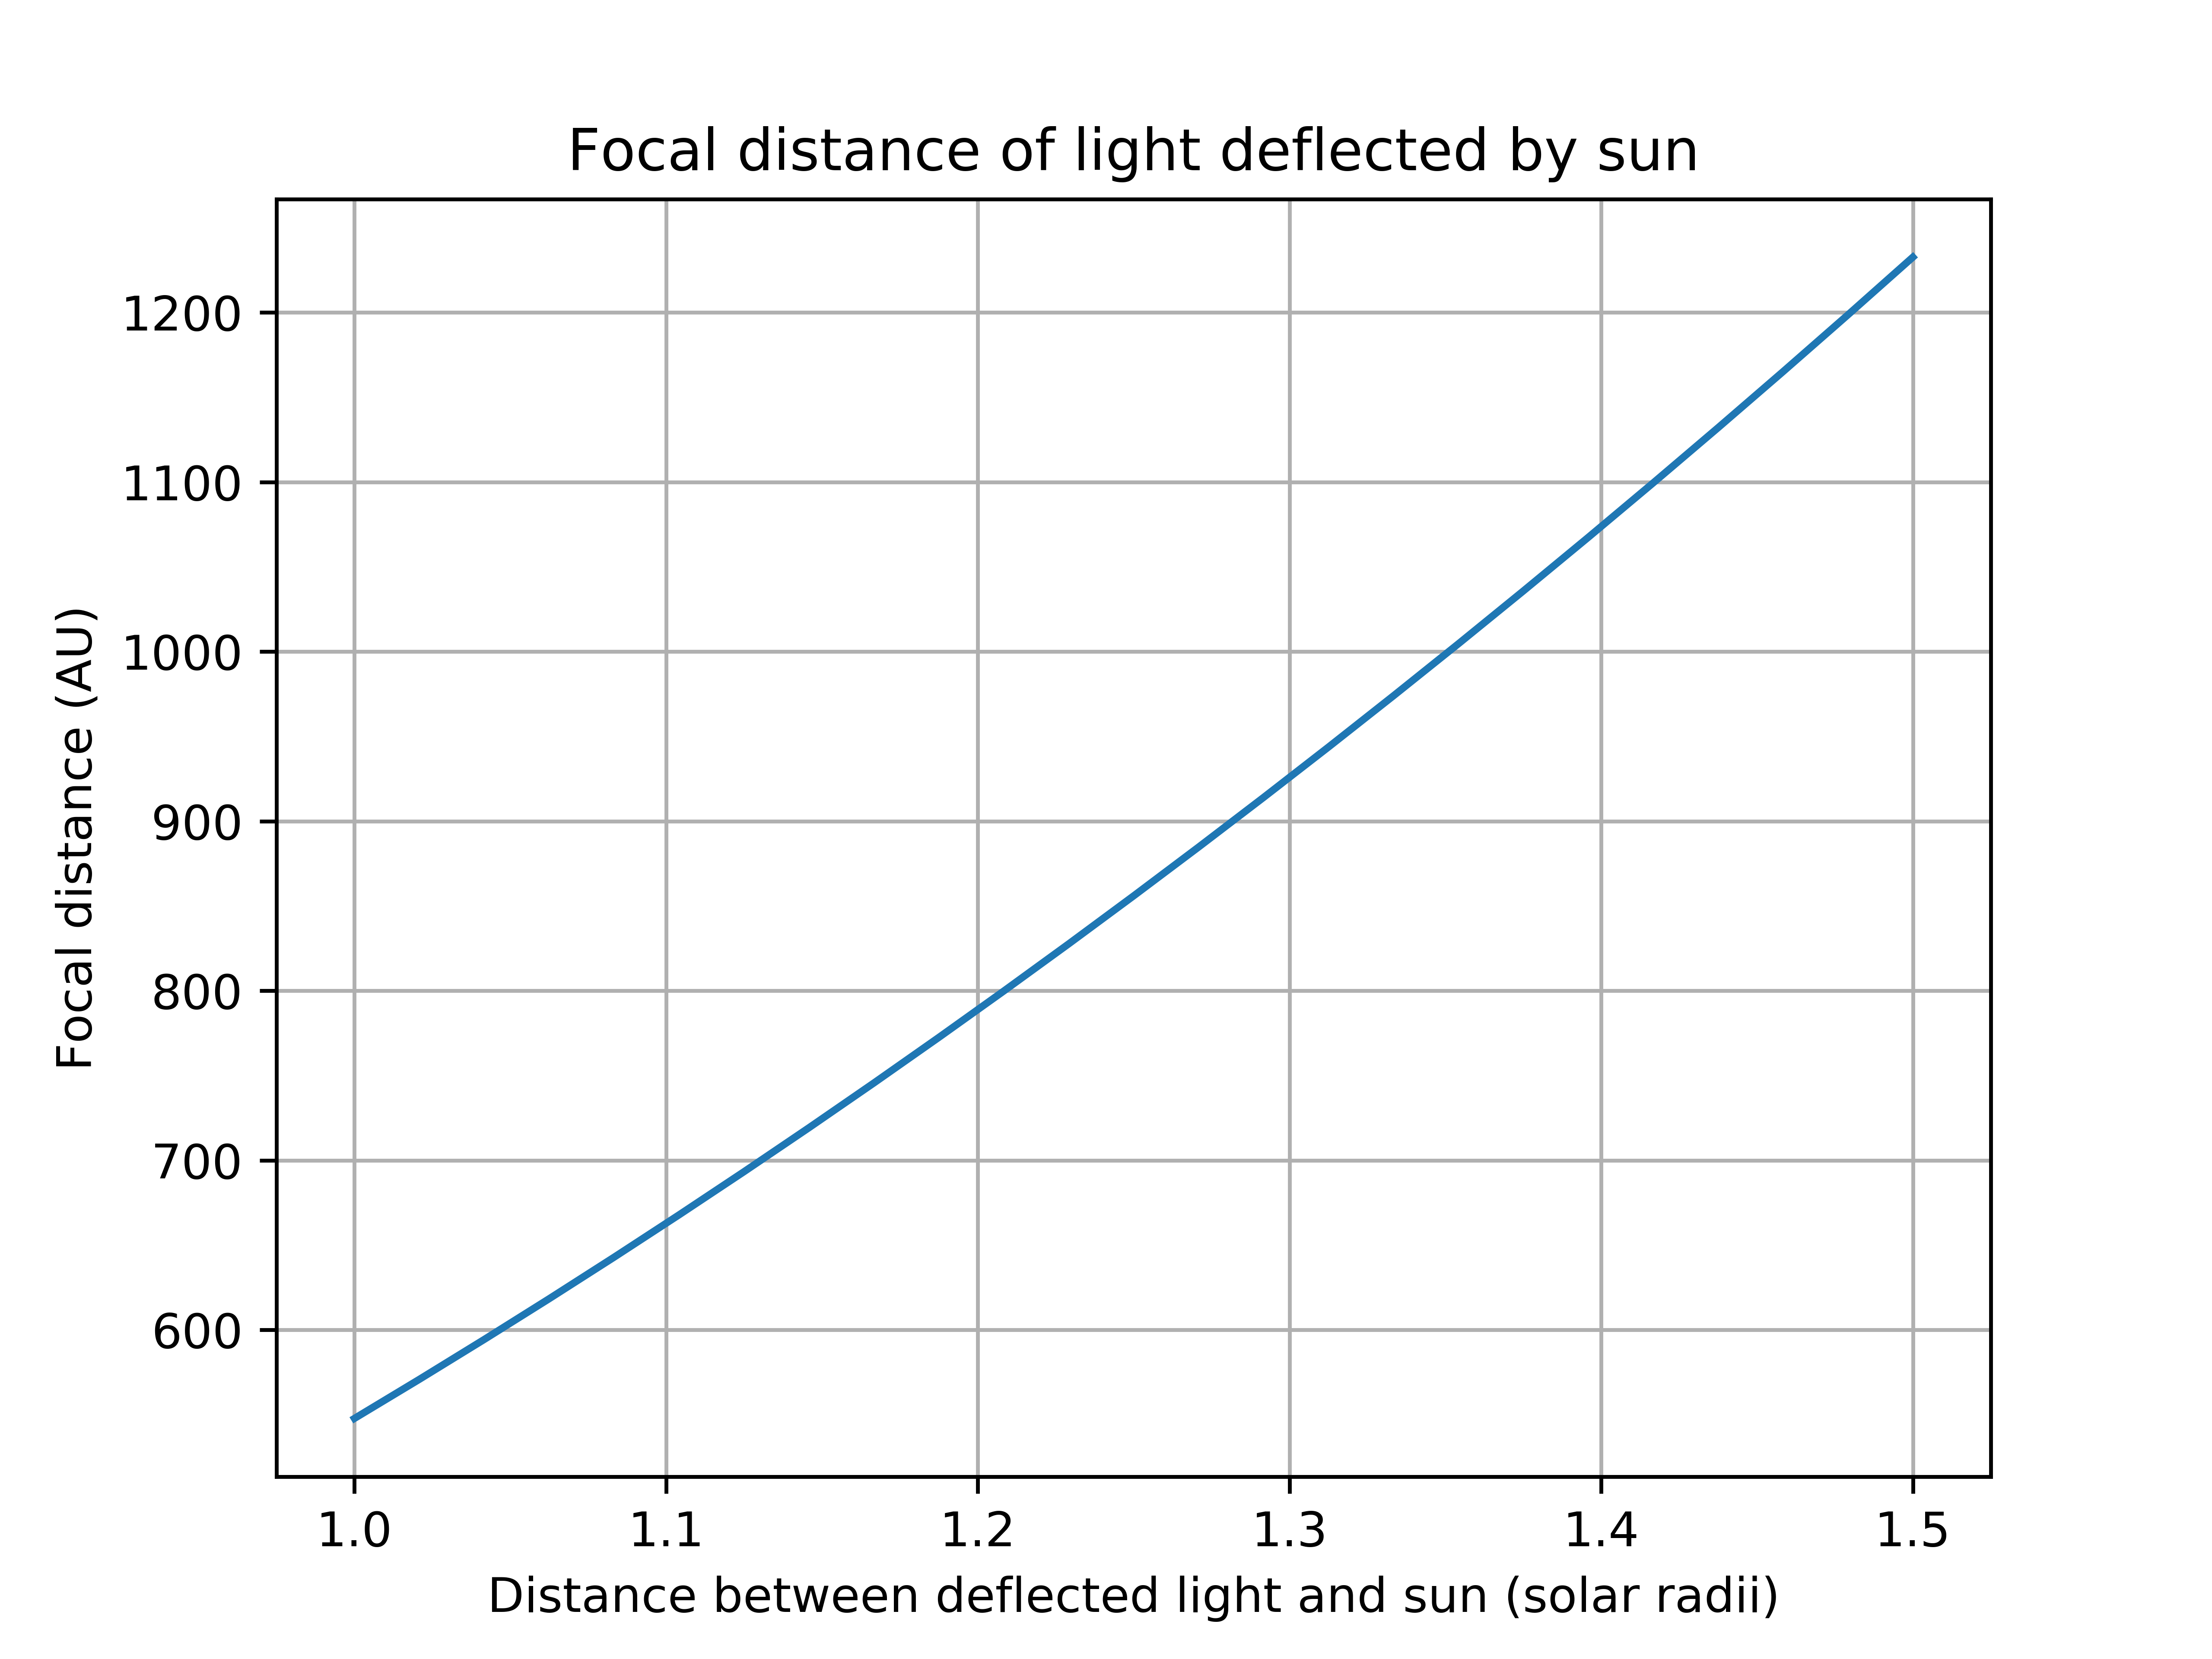
\includegraphics[width=5in]{image.png}}
\caption{Image of an Einstein ring LRG 3-757. The light from a distant galaxy is bent into a circle by the gravity of a closer, redder galaxy (center).}
\end{figure}

The equation for the deflection angle caused by the lens is:

$$\theta = \frac{4GM}{c^2r}$$

where:

$\theta$ is the angle of deflection\\
$G$ is the universal gravitational constant\\
$M$ is the mass of the lensing object (the sun)\\
$c$ is the speed of light\\
$r$ is the closest approach light takes the sun\\

The derivation of the equation is beyond the scope of this appendix.

The focal distance $f_d$ can be written as:

$$f_d = r\tan (\frac{\pi}{2} - \theta)$$
$$f_d = r\tan\bigg(\frac{\pi}{2} - \frac{4GM}{c^2r}\bigg)$$

The minimum focal distance comes from light passing close to the sun's surface, which minimizes r. For $r$ as the radius of the sun ($6.96 \times 10^8 m$):

$$f_d =  548AU$$

However, light passing so close to the sun would be difficult to separate from the sun itself. In the story a combination of a starshade and additional filtering is used to block light from the sun. A starshade is a flat, roughly circular plate that separates from \textit{Einstein} and flies nearby to block sunlight. The further the light passing by the sun is - corresponding to a larger $r$ - the further the \textit{Einstein} ring will be from the sun and the easier it is to photograph and interpret. Figure X below illustrates the relation between $r$ and the focal distance. 

\begin{figure}[H]
	\makebox[\textwidth][c]{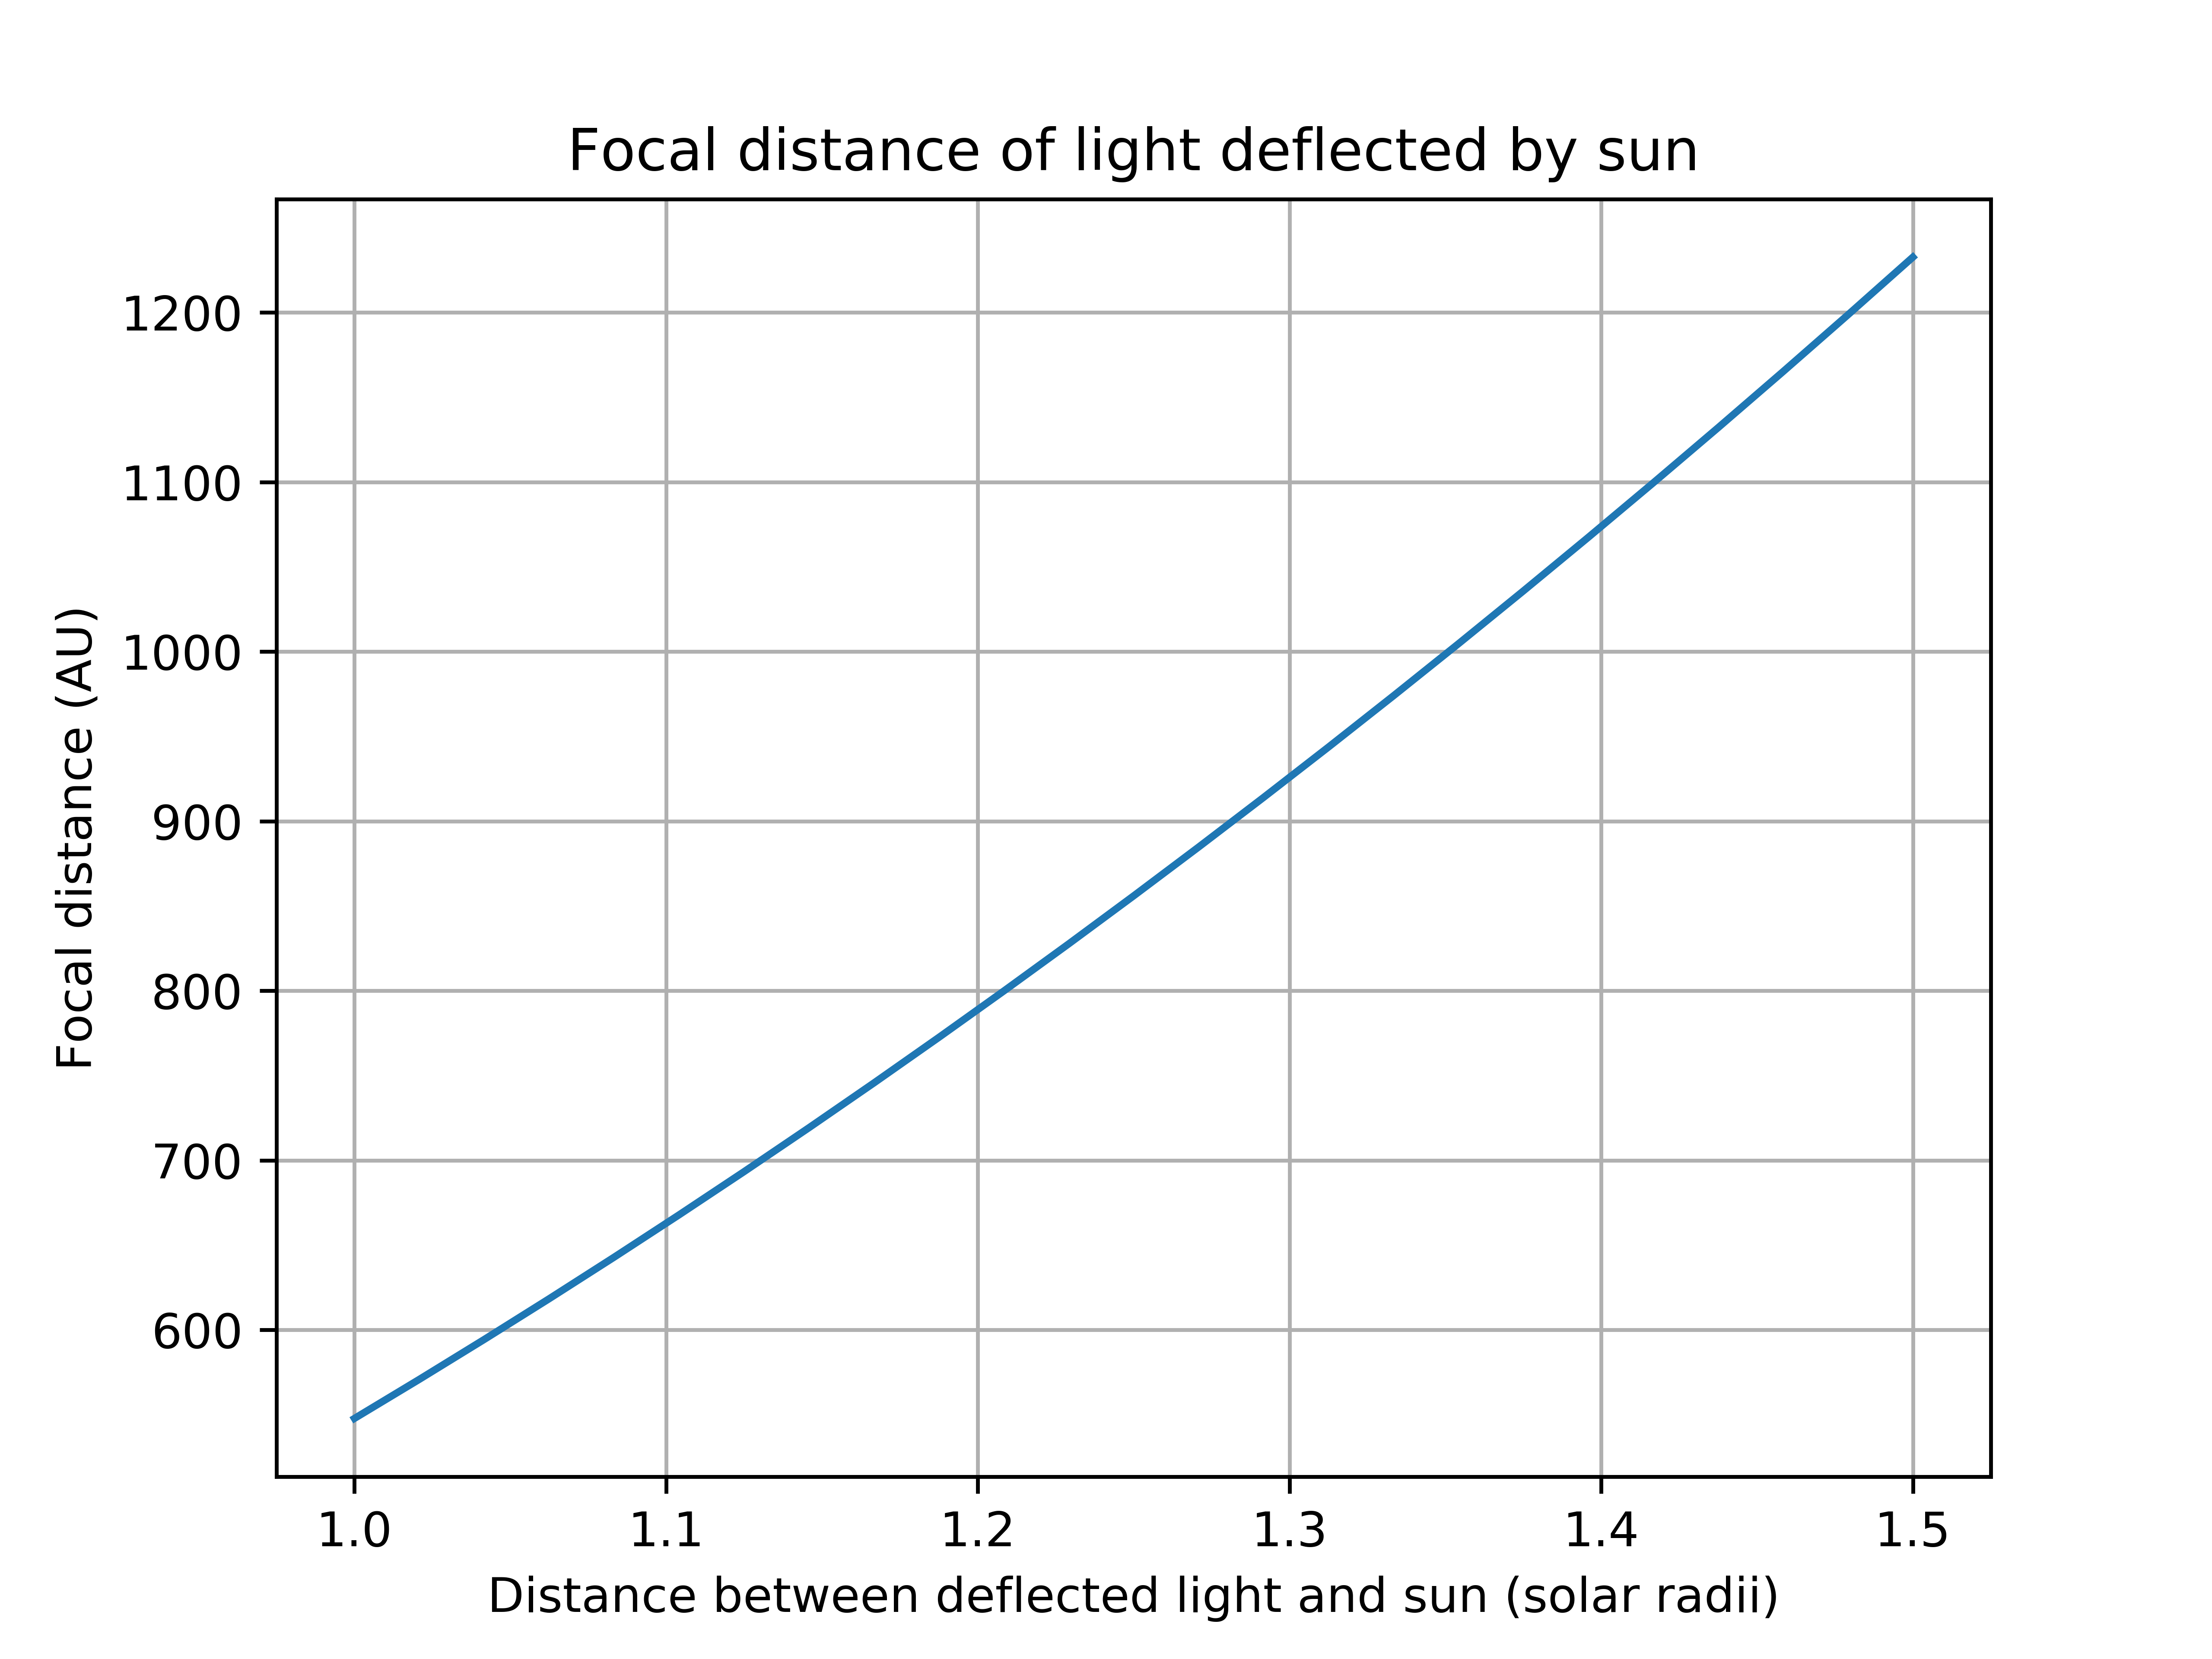
\includegraphics[width=5in]{image.png}}
	\caption{Focal distance as a function of how closely light from Trappist-1e passes to the sun. A greater focal distance takes longer to reach but leads to an \textit{Einstein} ring further from the sun that's easier to separate from the sun's light.}
\end{figure}

\textit{Einstein} must reach at least 548 AU to photograph an \textit{Einstein} ring of Trappist 1e. In practice, the telescope will need to travel than the minimum focal distance. As the telescope continues to coast through space and travel fruther from the sun the \text{Einstein} ring appears further from the sun. The total amount of light being bent into the ring also increases since the amount of light is proportional to the circumference of a circle around the sun with radius $r$. This means that the quality of images should improve as \textit{Einstein} travels further and further into space.

\section{Efficiency of \textit{Sheridan} drive}
\textit{Einstein} is powered by the \textit{Sheridan} drive, a closely guarded secret of the Callistan Navy. The drive is described as:

\hspace{2cm} \textit{a long sought after holy grail, a practical nuclear fusion engine}

This section will give some approximate specifications of the \textit{Sheridan} drive. Compared to other sections this section is lighter on detail and more speculative. Rather than attempt to sketch out the design of an actual nuclear fusion engine this section gives a general comparison between the \textit{Sheridan} drive and existing engines.

There are several choices of fuels for a nuclear fusion engine. The most likely are a deuterium tritium mix:
$$^2_1D^+ + ^3_1T^+ \rightarrow ^4_2He^{2+} (3.5 MeV) + n^0 (14.1 MeV)$$

or a helium-3 deuterium mix:

$$^2_1D^+ + ^3_2He^{2+} \rightarrow ^4_2He^{2+} (3.6 MeV) + p^+ (14.7 MeV)$$

Although the deuterium tritium reaction takes less energy to ignite, the helium-3 and deuterium mix is likely more favorable for a spacecraft engine. The byproducts of the second reaction are both charged and can be directed out of the engine bell by electromagnetic fields. The deuterium tritium reaction produces a neutral neutron which will be uniformly emitted in all directions. The neutron will also embed itself into the wall of the reactor, possibly embrittling and damaging the reactor.

The efficiency of an engine is related to its exhaust velocity. The exhaust velocity can be calculated from the kinetic energy:

$$E (joules) = \frac{1}{2}mv^2$$

Our energy units are in electron volts so the expression for velocity is:

$$v = \sqrt{\frac{2 E \frac{joules}{eV}}{m}}$$

for the helium-3 deuterim reaction this yields an exhaust velocity of:

$^4_2He^{2+}: 13,176 km/s$ or 0.044 c\\
$p^{+}: 53,059 km/s$ or 0.177 c\\

The exhuast of the \textit{Sheridan} drive is composed of two streams of particles with different exhaust velocities. The proton has an exhaust veloity of nearly 18\% the speed of light while the heavier alpha particle has a velocity of over 4\% the speed of light. The momentum change from the two exhaust streams is equivalent to the same mass being uniformly ejected at a velocity of:

$$p_{total} = 0.2mv_{p} + 0.8mv_{He} = mv_{combined}$$
$$v_{combined} = 0.2v_{p} + 0.8v_{He}$$
$$v_{combined} =  21,153km/s$$

which is equivalent to 7\% the speed of light. A common descriptor for the efficiency of an engine is its specific impulse, defined as the change in momentum per unit of fuel consumed.  When fuel is expressed by mass specific impulse is equivalent to exhaust velocity with units of meters per second. If weight is used then the units are expressed in seconds. The higher the exhaust velocity the greater the efficiency, and as we will see in the following section the faster a spacecraft can travel.

Since the \textit{Sheridan} drive is a first generation nuclear fusion engine we assume that its specific impulse is much less than the theoretical maximum. If we assume the specific impulse (and exhaust velocity) is an order of magnitude lower, then the specific impulse of the Sheridan drive is:

$$I_{sp} \approx 2,100 km/s \approx 214,000 seconds$$

Going forward we will round the \textit{Sheridan} drive's specific impulse to \textbf{200,000 seconds} and the exhaust velocity to \textbf{2,000} km/s.

The table below gives a comparison of the specific impulse of existing engines.

\begin{center}
\begin{tabular}{|m{5 cm}| m{5 cm}|} \hline
\textbf{Engine} & \textbf{Specific impulse (s)}\\ \hline
Falcon 9 Merlin-1D &  311 \\ \hline
Space shuttle main engine &  453 \\ \hline
Dawn ion engine   &  3100\\ \hline
\textit{Sheridan} drive & 200,000\\ \hline
\end{tabular}
\end{center}

The specific impulse of the \textit{Sheridan} drive is nearly two orders of magnitude greater than that of the \textit{Dawn} ion engines. We will see in the next section that the specific impulse is a strong driver of $\Delta v$, which in turn determines how long it takes \textit{Einstein} to reach the sun's focal point.

\section{\textit{Einstein} flight time}
In the story \textit{Einstein} takes ``decades" to reach the sun's focal point. This section calculates how long the trip takes based on the specific impulse of the \textit{Sheridan} drive and the distance to the focal point. Section 4 is more technically challenging than the first three sections and includes descriptions of several numerical approximations used to calculate \textit{Einstein}'s flight time.

The $\Delta v$ budget of a spacecraft is determined by the Tsiolkovsky rocket equation:

$$\Delta v = v_e ln \frac{m_0}{m_f}$$

where:

$v_e$ is exhaust velocity\\
$m_0$ is the starting mass\\
$m_f$ is the ending mass after all fuel is expended\\

The $\Delta v$ strongly depends on the fraction of the spacecraft taken up by fuel. For \textit{Einstein} we assume that the exhaust velocity is 2,000 km/s and that the fraction of the starting mass taken up by fuel is 10\%. For comparison, NASA's \textit{Cassini-Huygens} probe was more than 50\% fuel at launch. Since \textit{Einstein} is a first generation nuclear fusion engine with a heavy reactor we assume it has a lower fuel ratio. Substituting into the rocket equation gives a $\Delta v$ of:

$$\Delta v = 2,000,000\frac{m}{s} \times ln \frac{1}{0.9}$$
$$\Delta v \approx 210 km/s$$ 

During its flight to the focal point \textit{Einstein} can change its velocity by 210 km/s. Put another way, it has a $\Delta v$ budget of 210km/s.The flight to the focal point can be broken into several phases:
\begin{enumerate}
\item Jupiter approach burn
\item Jupiter escape burn
\item Coast to perihelion
\item Perihelion burn
\item Coast to focal point
\end{enumerate}

Each burn requires a certain $\Delta v$ to execute. In the following subsections we will add up how much time each of the four phases takes and how much of the $\Delta v$ budget is expended.

\subsection{Jupiter approach burn}
In the story \textit{Einstein} is launched from Callisto first into a parking orbit around the moon. Afterwards, the telescope is launched on a trajectory that brings it close to Jupiter. Figure X illustrates the trajectory \textit{Einstein} takes.

\begin{figure}[H]
	\makebox[\textwidth][c]{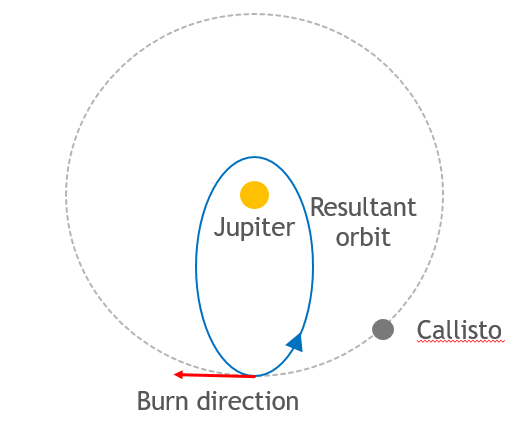
\includegraphics[width=3.8in]{jupiter_approach.png}}
	\caption{Illustration of \textit{Einstein}'s orbit around Jupiter after launching from Callisto. The launch vehicle puts the telescope on a trajectory that brings it close to Jupiter (figure not to scale).}
\end{figure}

For several reasons we will not include the $\Delta v$ of the Jupiter approach burn or the time it takes to reach Jupiter into our calculations.

The transit time from Callisto to Jupiter is on the order of several days to a few weeks (for comparison Callisto's orbital period is 17 days). Since the time needed to escape from Jupiter is relatively small compared to the years \textit{Einstein} spends coasting to the sun we will ignore the time when calculating total flight time.

In the story the rocket that launches \textit{Einstein} also sends it on a trajectory that takes it close to Jupiter. Since \textit{Einstein} isn't expending any fuel to make its dive toward Jupiter, we will not include the $\Delta v$ of the Jupiter approach burn in our calculations.

$\Delta$ \textbf{v:} 0 km/s\\
\textbf{Time:} 0

\subsection{Jupiter escape burn}
The second leg of the trip is to escape from Jupiter's gravity well. After \textit{Einstein} is launched from Callisto it flies on an elliptical orbit that takes it near Jupiter. When the craft is near Jupiter the \textit{Sheridan} drive performs its first burn to escape from Jupiter's gravity well and put it on a trajectory close to the sun. Figure x illustrates \textit{Einstein}'s trajectory as it executes the Jupiter escape burn.

\begin{figure}[H]
	\makebox[\textwidth][c]{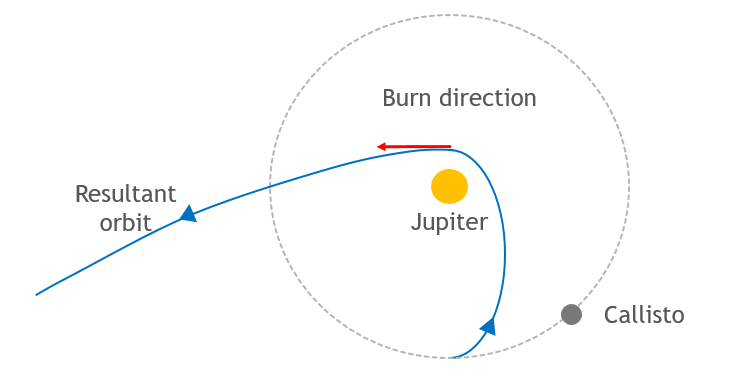
\includegraphics[width=5in]{jupiter_escape.png}}
	\caption{Illustration of \textit{Einstein}'s orbit around Jupiter. When the telescope is at its closest approach the \textit{Sheridan} performs the Jupiter escape burns to send the spacecraft on a trajectory leaving Jupiter and into a heliocentric orbit.}
\end{figure}

In section 1 of the appendix we calculated that a $\Delta v$ of about 10 km/s is needed to put \textit{Einstein} on a trajectory taking it close to the sun. This is the velocity relative to Jupiter; it means that when \textit{Einstein} is performing the Jupiter escape burn it must have a v-infinity relative to Jupiter of 10km/s. From section 1 we know the expression for v-infinity is:

$$v_{\infty} = \sqrt{(v_p + \Delta v_2)^2-\frac{2MG}{r_p}}$$

Where:
$v_0$: starting velocity\\
$\Delta v$: change in velocity supplied by \textit{Sheridan} drive\\
$r_p$: starting distance from Jupiter

We assume that $r_p$ is 75,600km, the same distance from the center of Jupiter that NASA's \textit{Juno} probe will reach on its closest approach. Knowing that \textit{Einstein} started at Callisto's orbit, we can calculate $v_p$ using the equation for specific orbital energy seen earlier:

$$\frac{1}{2}v^2-\frac{MG}{r} = -\frac{MG}{2a}$$

where:\\
$a: r_p + r_a$
$r = r_p: 7.56\times 10^7m$\\
$r_a:$ orbital distance of Callisto $1.88 \times 10^9$m\\
$M:$ mass of Jupiter $1.90\times10^27$\\


substituting gives us \textbf{$v_p = 57.3 km/s$}

Plugging the values for $v_p$, $v_{\infty}$, and $r_p$ into the equation for $v_{\infty}$ above gives us \textbf{$\Delta v = 1.5km/s$}.

It only takes a small $\Delta v$ to escape from Jupiter because \textit{Einstein} starts from a highly eccentric orbit. Burning at perijove (the point closest to Jupiter) takes advantage of the Oberth effect and allows \textit{Einstein} to have a high v-infinity while using little fuel.

Like in the previous section, we will ignore the time it takes \textit{Einstein} to escape from Jupiter's gravity well because the time is relatively short compared to the rest of the flight. 


$\Delta$ \textbf{v:} 1.5 km/s\\
\textbf{Time:} 0

\subsection{Coast to perihelion}
The second leg of the trip is when \textit{Einstein} coasts from Jupiter inwards towards the sun. The spacecraft follows an elliptical orbit and does not expend any fuel. We will use Kepler's law to calculate how long it takes \textit{Einstein} to coast from Jupiter's orbit to its closest approach to the sun. The period of an orbit is given by Kepler's second law:

$$T^2 \propto a^3$$

which states that the period of an orbit squared is proportional to the semi major axis cubed. The earth has a period of one year and a semi-major axis of almost exactly one AU. Using the units of years and AU the ratio between period squared and semi-major axis cubed is one.

The elliptical orbit that \textit{Einstein} takes has a semi-major axis of:

$$a = \frac{1}{2}(r_{perihelion} + r_{aphelion})$$

where\\
$r_{perihelion}:$ closest approach to the sun = 0.1 AU\\
$r_{aphelion}:$ furthest distance to the sun = 5 AU\\

The perihelion is limited by how close \textit{Einstein} can be to the sun without overheating. For comparison NASA's Parker Solar Probe, which has specially designed thermal protection, will fly within 0.046 AU of the sun. Substituting into Kepler's law gives a period of:

$$1 = \frac{T^2}{a^3}$$
$$2.05AU^{3} = T^2$$
$$T = 4.1 years$$

The period of \textit{Einstein}'s elliptical trajectory is about 4 years. The time it takes \textit{Einstein} to complete half an orbit (starting from the aphelion and ending at perihelion) is half that, or about 2 years.

$\Delta$ \textbf{v:} 0 km/s\\
\textbf{Time:} 2 years

% Perihelion burn
\subsection{Perihelion burn}
The burn at perihelion is the \textit{Sheridan} drive's longest and most powerful burn. In the story the engine burns continuously for several days, accelerating \textit{Einstein} out of the solar system. In this section we'll calculate \textit{Einstein}'s v-infinity after performing the burn. We're going to make two approximations that will make calculations much easier while giving us a reasonably accurate answer:

\begin{enumerate}
\item \textit{Einstein}'s trajectory is a straight line that starts at the perihelion and continues perpendicular to a line connecting the perihelion to the sun.
\item The long, multi day burn is approximated as a series of discrete, instantaneous velocity changes (step burns) separated by periods when \textit{Einstein} cruise. During the cruise phases \textit{Einstein}'s velocity is governed only by the effect of gravity.
\end{enumerate}

In reality, \textit{Einstein} follows a hyperbolic path that constantly changes as the burn continues. The approximation underestimates the final v-infinity because the straight path moves away from the sun more quickly than a hyperbolic path that curves slightly inwards towards the sun. Leaving the sun's gravity well more quickly reduces the Oberth effect, and leads to a lower v-infinity. However, it is still a \textit{fairly} good approximation. Figure X below illustrates how the approximated trajectory compares to a more \textit{Einstein}'s actual path.

\begin{figure}[H]
	\makebox[\textwidth][c]{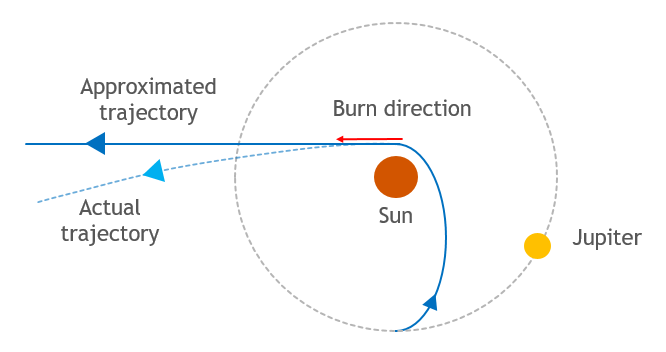
\includegraphics[width=5in]{solar_escape.png}}
	\caption{Comparison of \textit{Einstein}'s actual trajectory and the approximated trajectory. Figure not drawn to scale.}
\end{figure}

In our approximation, \textit{Einstein}'s velocity will have a sawtooth pattern as it flies away from the sun. Each burn is equally spaced in time and increases the spacecraft's velocity instantaneously. During the cruise periods \textit{Einstein}'s velocity falls off slightly as it flies away from the sun.

\begin{figure}[H]
	\makebox[\textwidth][c]{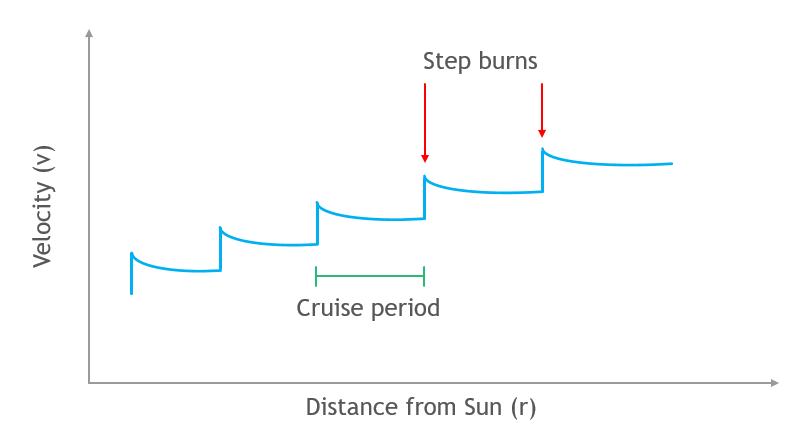
\includegraphics[width=5in]{einstein_velocity.png}}
	\caption{Illustration of \textit{Einstein}'s approximated velocity as it flies away from the sun. Instead of constantly accelerating, in our approximation we instantaneously increase the telescope's velocity through a series of step burns. The combined $\Delta v$ of the step burns is equivalent to the $\Delta v$ of the solar escape burn. Between the burns the velocity drops as \textit{Einstein} coasts away from the sun. The time between each step burn is kept constant, resulting in the distance between each step burn increasing as the velocity increases. Graph not drawn to scale.}
\end{figure}

We will use the following steps to approximate the telescope's velocity after it's perihelion burn:

\begin{enumerate}
\item Divide the $\Delta v$ of the perihelion burn by the number of steps to get the $\Delta v$ of each \textbf{step burn}.
\item Divide the how long the perihelion burn is by the number of steps to get the \textbf{step cruise time}. 
\item Instantaneously increase the velocity by the $\Delta v$ of the step burn.
\item Use a linear approximation to estimate how far \textit{Einstein} should coast for so that the coast time is equal to the step cruise time.
\item Update \textit{Einstein}'s position and velocity after the cruise phase as it coasts on a straight line. The time spent during each cruise phase between the step burns should equal the step cruise time.
\item Repeat steps 2-5 until the burn and the total velocity change is complete. This breaks the continuous, multi-day burn into many small burns.
\end{enumerate}

The first three steps are straightforward - we're calculating how large each step burn is and how long the cruise step time between each burn should be to maintain a constant average acceleration.

Step 4 is the most sophisticated step. The goal of this step is to calculate \textit{how far} \textit{Einstein} needs to coast during each cruise period so that the \textit{time it takes to coast that distance} is equal to the step cruise time. Since \textit{Einstein}'s velocity changes as it flies away from the sun, the distance it travels during each cruise phase also changes. Calculating the distance traveled during each cruise phase let's us update \textit{Einstein}'s position and velocity before the next step burn.

\subsubsection{Step 4: Creating a linear approximation}
The goal of step 4 is to find what \textit{Einstein}'s new position and velocity are after it coasts for the step cruise time following a step burn.

The relation between cruise time and cruise distance is given by: 

$$T = \int_{x_0}^{x_f} \frac{1}{v(x)} dx$$

where:\\
$x_0$: starting distance traveled from perihelion\\
$x_f$: ending distance traveled from perihelion\\
$v(x)$: velocity as a function of distance from perihelion\\
$T$: time elapsed - cruise step time\\

The cruise distance is equal to $x_f - x_0$.

If we can solve for this integral analytically, we can rearrange it and get an explicit formula for the cruise distance as a function of time. Updating \textit{Einstein}'s position is then simply plugging in the desired cruise time between burns and calculating its new position. However, as we will see this integral cannot be solved analytically.

The equation for velocity as a function of distance from the sun $r$ comes from the equation for specific orbital energy. Since the telescope is coasting, the sum of its kinetic and potential energy is constant:

$$\frac{1}{2}v_0^2-\frac{M_sG}{r_0} = \frac{1}{2}v(r)^2-\frac{M_sG}{r}$$
$$v(r) = \sqrt{2  (\frac{1}{2}v_0^2-\frac{M_sG}{r_0} + \frac{M_sG}{r})}$$
$$v(r) = \sqrt{v_0^2-\frac{2M_sG}{r_0} + \frac{2M_sG}{r}}$$

This expression gives the velocity as a function of $r$ the distance from the sun. However, we need an expression for velocity as a function of $x$, the distance traveled from the perihelion. 

Using the relation:

$$r^2 = x^2 + r_p^2$$

where $r_p$ is the perihelion distance gives us:

$$v(x) = \sqrt{v_0^2-\frac{2M_sG}{\sqrt{x_0^2 + r_p^2}} + \frac{2M_sG}{\sqrt{x^2 + r_p^2}}}$$

Substituting this equation into the equation for time gives an integral that cannot be solved analytically. Instead, we can use a linear approximation for the velocity as a function of distance:

$$v(x) \approx v_0 + v'(x_0)x$$

Substituting the linear approximation into the time integral gives:

$$\boxed{T = \int_{x_0}^{x_f} \frac{1}{v_0+v'(x_0)x} dx}$$

where:\\
$v_0$= velocity at the beginning of the cruise phase\\
$x_0$: starting distance traveled from perihelion\\
$x_f$: ending distance traveled from perihelion\\
$v(x)$: velocity as a function of distance from perihelion\\
$T$: time elapsed - cruise step time\\

Going forward, we will solve this integral and use a linear approximation for \textit{Einstein}'s velocity.

\subsubsection{Solving for cruise distance as a function of time}

Now that we have the form of a linear approximation for velocity, we need to create an expression for the cruise distance $(x_f-x_0)$ as a function of time ($T$).

Using $m$ for the derivative of velocity at $x_0$:

$$m = \frac{dv}{dx}(x_0)$$

we can solve for the integral using $u$ substitution:

$$T = \int_{x_0}^{x_f} \frac{1}{v_0+mx} dx$$
$$u = v_0+mx\hspace{10mm}du = mdx\hspace{10mm}dx = \frac{1}{m}du$$
$$T = \int \frac{1}{u} \frac{1}{m}dx$$
$$T = \frac{1}{m} \log{u}$$
$$T = \frac{1}{m} \log{(v_0+mx)}\bigg]_{x_0}^{x_f}$$
$$T = \frac{1}{m} \bigg(\log{(v_0+mx_f)} - \log{(v_0+mx_0)}\bigg)$$

We want an expression for the \textbf{final position $(x_f)$} of \textit{Einstein} after it cruises for a given step cruise time  $(T)$ so we rearrange the equation:

$$mT = \log{(v_0+mx_f)} - \log{(v_0+mx_0)}$$
$$\log{(v_0+mx_f)} = \log{(v_0+mx_0)} + mT$$
$$v_0 + mx_f = e^{\log{(v_0+mx_0)}+mT}$$
$$v_0 + mx_f = e^{mT}(v_0+mx_0)$$
$$mx_f = e^{mT}(v_0+mx_0) - v_0$$
$$\boxed{x_f = \frac{1}{m}\bigg(e^{mT}(v_0+mx_0) - v_0\bigg)}$$


The only piece of this equation we're missing is an expression for $m$, the slope of the velocity as a function of distance traveled from the perihelion $x$. 

\subsubsection{Calculating $v'(x_0)$}

For the equation in the above section we need to solve for $m$, which we've defined as $v'(x_0)$. We can solve for this by taking the derivative of $v(r)$ with respect to $r$ and applying the chain rule:

$$\frac{dv}{dx} = \frac{dv}{dr}\times\frac{dr}{dx}$$

From an earlier section we derived the expression for $v(r)$:

$$v(r) = \sqrt{v_0^2-\frac{2M_sG}{r_0} + \frac{2M_sG}{r}}$$

Solving for $\frac{dv}{dr}$:

$$\frac{dv}{dr} = \frac{1}{2} \bigg(v_0^2-\frac{2M_sG}{r_0} + \frac{2M_sG}{r}\bigg)^{-\frac{1}{2}}\frac{dv}{dr}\bigg(v_0^2-\frac{2M_sG}{r_0} + \frac{2M_sG}{r}\bigg)$$

$$\frac{dv}{dr} = \frac{1}{2} \bigg(v_0^2-\frac{2M_sG}{r_0} + \frac{2M_sG}{r}\bigg)^{-\frac{1}{2}}2M_sG\log{r}$$

$$\frac{dv}{dr} = \frac{2M_sG \log{r}}{2 \sqrt{v_0^2-\frac{2M_sG}{r_0} + \frac{2M_sG}{r}}}$$

$$\frac{dv}{dr} = \frac{M_sG \log{r}}{ \sqrt{v_0^2-\frac{2M_sG}{r_0} + \frac{2M_sG}{r}}}$$

The expression for $\frac{dv}{dr}$ quickly becomes complicated and we still need to use the chain rule to reach $\frac{dv}{dx}$. Instead of explicitly calculating the derivative, we can approximate the derivative by calculating the velocity at two points and solving for the slope:

$$\frac{dv}{dx} \approx \frac{v(x_0 +\Delta) - v(x_0)}{\Delta}$$

Using this equation and plugging in a small $\Delta$ will give us a good estimate for the slope. At the beginning of the cruise phase we know the initial velocity, $v(x_0)$. We can calculate the velocity at the second point $v(x_0 + \Delta)$ by using conservation of specific orbital energy, expressed by our equation for $v(r)$:

$$v(r) = \sqrt{v_0^2-\frac{2M_sG}{r_0} + \frac{2M_sG}{r}}$$

and using the relation between $r$, $x$, and $r_p$:

$$r^2 = x^2 + r_p^2$$


\subsubsection{Calculating the result}
To recap, the goal of creating a linear approximation was to estimate the \textbf{how far \textit{Einstein} coasts} during the set step cruise time. Knowing the cruise distance let's us update the spacecraft's position and velocity at the end of each cruise  phase. To solve for time we used two steps:
\begin{enumerate}
\item Calculate the slope of the velocity as a function of distance traveled immediately after the step burn
\item Plug the time, the slope, the initial velocity, and the initial position into the expression for the final position:

$$\boxed{x_f = \frac{1}{m}\bigg(e^{mT}(v_0+mx_0) - v_0\bigg)}$$

We arrived at this solution by rearranging the integral:
$$\boxed{T = \int_{x_0}^{x_f} \frac{1}{x_0+v'(x_0)x} dx}$$
\end{enumerate}

We repeat this process until the sum of the step burns equals the $\Delta v$ of the total perihelion escape burn. To view the Python program used to perform this calculation, please visit:

\url{github.com/timsliu/flybys_foci/flight_time.py}

Using the following inputs:

\begin{center}
\begin{tabular}{|m{5 cm}| m{5 cm}| m{5 cm}|} \hline
\textbf{Parameter} & \textbf{Value} & \textbf{Units}\\ \hline
n & 1000& steps\\ \hline
$\Delta v$ & 200& km/s \\ \hline
$r_p$      &  0.1& AU\\ \hline
$v_p$     &  & km/s\\ \hline
Total perihelion burn time & 10 & days \\ \hline
Step burn $\Delta v$ & 200 & m/s\\ \hline
Step cruise time & 864& seconds \\ \hline
\end{tabular}
\end{center}

yields the final orbital parameters for \textit{Einstein} after its perihelion burn:

\begin{center}
\begin{tabular}{|m{5 cm}| m{5 cm}| m{5 cm}|} \hline
\textbf{Parameter} & \textbf{Value} & \textbf{Units}\\ \hline
Position (x) & a& km from perihelion\\ \hline
Radial distance (r) & a& km from the sun\\ \hline
Velocity      &  a& km/s\\ \hline
v-infinity     &  a& km/s\\ \hline
\end{tabular}
\end{center}

A 200 km/s escape burn spread over 10 days (an average acceleration of $0.23m/s^2$) increases \textit{Einstein}'s velocity to xx. At the end of the burn the spacecraft is xx AU from the sun, or xx the orbit of Mercury.


$\Delta$ \textbf{v:} 200 km/s\\
\textbf{Time:} 10 days\\

\subsection{Coast to focal point}
After its final burn \textit{Einstein} makes an unpowered coast to the focal point. This is the longest leg of the telescope's journey. As the spacecraft flies further from the sun it slows down, exchanging kinetic energy for potential energy. The velocity of \textit{Einstein} as a function of its distance from the sun $r$ is equivalent to its total specific orbital energy at the end of its perihelion burn:

$$E_{b} = \frac{1}{2}v_b^2 - \frac{MG}{r_b} = \frac{1}{2}v^2-\frac{MG}{r}$$
$$\frac{1}{2}v^2 = E_b+\frac{MG}{r}$$
$$\boxed{v = \sqrt{2\big(E_b + \frac{MG}{r}\big)}}$$

Where:

$E_b$ is the specific orbital energy after the perihelion burn\\
$v_b$ is the spacecraft velocity after the perihelion burn\\
$r_b$ is the spacecraft distance from the sun after the perihelion burn\\

Figure X plots the velocity of \textit{Einstein} as a function of distance from the sun.

To calculate \textit{Einstein}'s flight time we again need to solve the integral:

$$T = \int_{r_0}^{r_f} \frac{1}{v(r)} dr$$

This is the reverse of the problem we had in the previous section. In the last section we needed to solve for a distance that \textit{Einstein} travels during the step cruise time. Now we are solving for the time it takes \textit{Einstein} to coast a certain distance - to the suns focal point. We will evaluate this integral where:

$r_0 = r_b$: spacecraft distance from the sun after the perihelion burn\\
$r_f$: focal distance of the sun\\
$v(r)$ the expression for velocity derived above.

As we saw in the previous section, this integral cannot be solved analytically. Instead, we use Simpson's rule to approximate:

$$\int_a^b f(x) dx \approx \frac{\Delta x}{3} (f(x_0) + 4f(x_1)+ 2f(x_2) + 4f(x_3) + 2 f(x_4) + ... + 4f(x_{n-1}) + f(x_n))$$

The Python program used for numerically evaluating this integral can be found at 

\url{github.com/timsliu/flybys_foci/flight_time.py}

Using a step size $\Delta x$ of x we get a flight time of xx years from $r_b$ to the focal point. Adding the time \textit{Einstein} spent coasting from Jupiter to the perihelion gives us a \textbf{total estimated flight time of xx years}. This is the time it takes for \textit{Einstein} to just reach the beginning of the sun's focal point - as it continues to coast it stays on the sun's focal line where the magnification steadily becomes stronger. The figure below plots the distance from the sun \textit{Einstein} reaches as a function of flight time.

\begin{figure}[H]

	\caption{\textit{Einstein}'s distance from the sun as a function of flight time.}
\end{figure}

\subsection{Additional considerations}
Several major simplifications were made when calculating \textit{Einstein}'s flight time. One of the most prominent is that orbital inclination was ignored.


We calculated the time it would take \textit{Einstein} to reach the sun's focal point. However, to actually observe a planet a gravitionally lensing telescope can't fly in any direction - it must reach the sun's focal point \textit{and} be aligned with the sun and the target planet. If the target star is not aligned with the ecliptic - a plane in space defined by the Earth's orbit - then a spacecraft must perform an additional burn. The added burn changes the spacecraft's orbital inclination, the angle between the plane of the orbit and the ecliptic. Changing the orbital inclination sends a spacecraft either above or below the plane of planets orbiting the sun.

Luckily, Trappist-1 sits at an inclination of xx relative to the sun. This is a fairly small orbital inclination and can be adjusted by the flyby of Jupiter. Targeting the flyby to pass over the poles of Jupiter sends \textit{Einstein} on a trajectory either above or below the ecliptic (depending on whether the orbit passes south to north or north to south). Adjusting the flyby is an easy way to send \text{Einstein} on a trajectory with the right orbital inclination without needing much more fuel.

\section{References}






\end{document}
